\documentclass{standalone}
\usepackage{tikz}
\usetikzlibrary{patterns, positioning}

\begin{document}
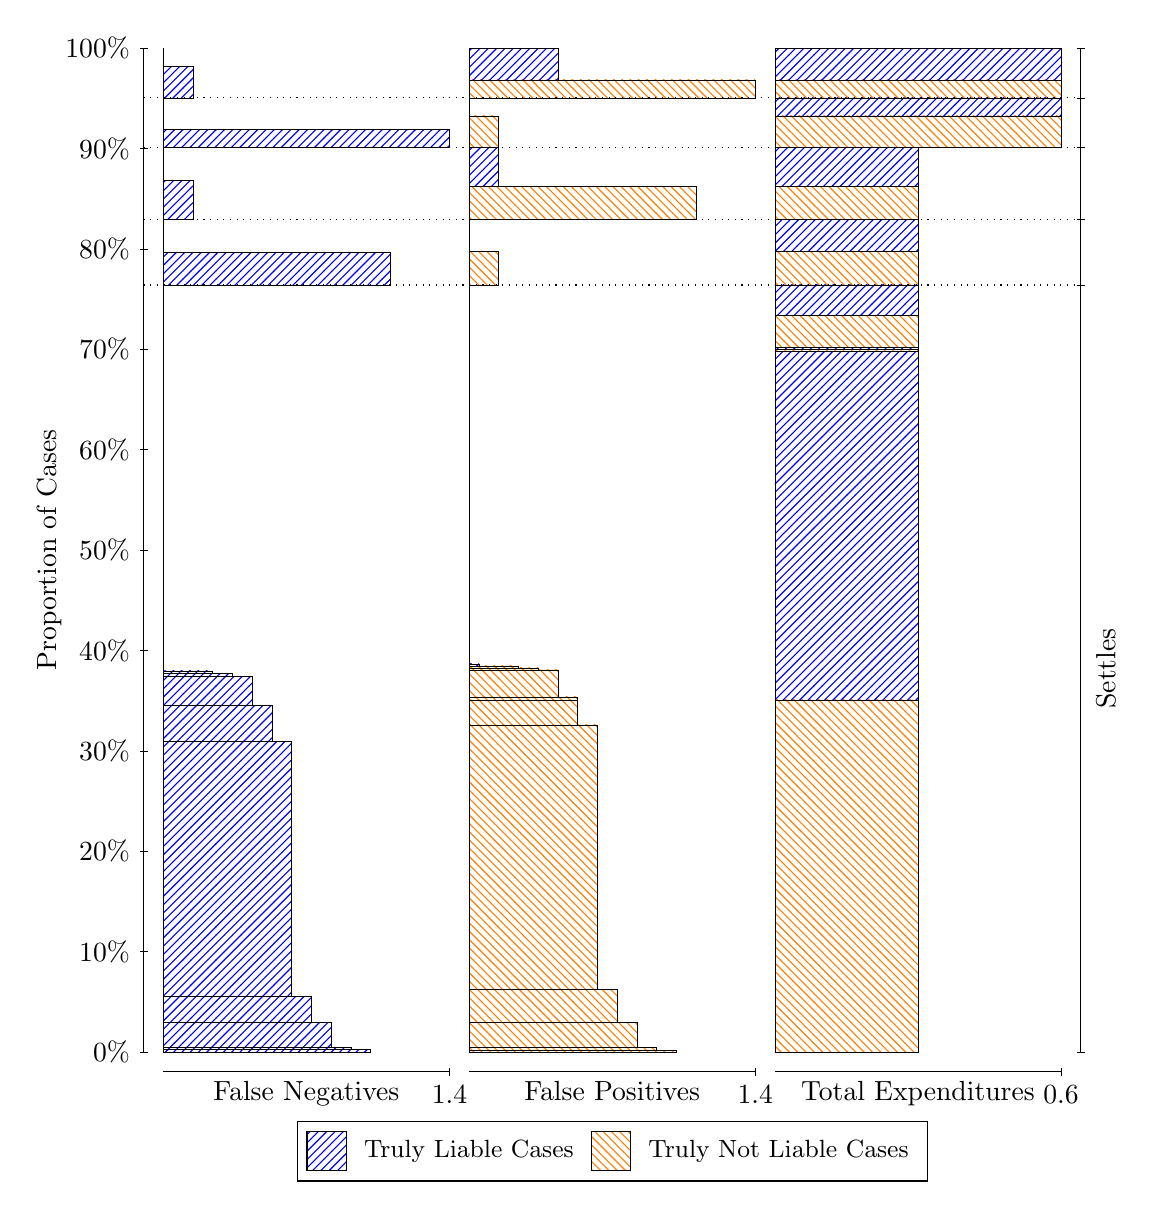
\begin{tikzpicture}
\draw[black, very thin] (1.5,1.75) -- (1.5,14.5);
\node[rotate=90, anchor=center] at (0.3, 8.125) {Proportion of Cases};
\draw[black, very thin] (1.45,1.75) -- (1.55,1.75);
\node[anchor=east] at (1.45, 1.75) {0\%};
\draw[black, very thin] (1.45,3.025) -- (1.55,3.025);
\node[anchor=east] at (1.45, 3.025) {10\%};
\draw[black, very thin] (1.45,4.3) -- (1.55,4.3);
\node[anchor=east] at (1.45, 4.3) {20\%};
\draw[black, very thin] (1.45,5.575) -- (1.55,5.575);
\node[anchor=east] at (1.45, 5.575) {30\%};
\draw[black, very thin] (1.45,6.85) -- (1.55,6.85);
\node[anchor=east] at (1.45, 6.85) {40\%};
\draw[black, very thin] (1.45,8.125) -- (1.55,8.125);
\node[anchor=east] at (1.45, 8.125) {50\%};
\draw[black, very thin] (1.45,9.4) -- (1.55,9.4);
\node[anchor=east] at (1.45, 9.4) {60\%};
\draw[black, very thin] (1.45,10.675) -- (1.55,10.675);
\node[anchor=east] at (1.45, 10.675) {70\%};
\draw[black, very thin] (1.45,11.95) -- (1.55,11.95);
\node[anchor=east] at (1.45, 11.95) {80\%};
\draw[black, very thin] (1.45,13.225) -- (1.55,13.225);
\node[anchor=east] at (1.45, 13.225) {90\%};
\draw[black, very thin] (1.45,14.5) -- (1.55,14.5);
\node[anchor=east] at (1.45, 14.5) {100\%};

\draw[black, very thin] (13.4,1.75) -- (13.4,14.5);
\draw[black, very thin] (13.35,1.75) -- (13.45,1.75);
\node[anchor=west] at (13.35, 1.75) {};
\draw[black, very thin] (13.35,11.491) -- (13.45,11.491);
\node[anchor=west] at (13.35, 11.491) {};
\draw[black, very thin] (13.35,12.324) -- (13.45,12.324);
\node[anchor=west] at (13.35, 12.324) {};
\draw[black, very thin] (13.35,13.234) -- (13.45,13.234);
\node[anchor=west] at (13.35, 13.234) {};
\draw[black, very thin] (13.35,13.867) -- (13.45,13.867);
\node[anchor=west] at (13.35, 13.867) {};
\draw[black, very thin] (13.35,14.5) -- (13.45,14.5);
\node[anchor=west] at (13.35, 14.5) {};

\draw[black, very thin, pattern color=blue, pattern=north east lines] (1.75,1.75) rectangle (4.381,1.7786);
\draw[black, very thin, pattern color=blue, pattern=north east lines] (1.75,1.7786) rectangle (4.1305,1.8075);
\draw[black, very thin, pattern color=blue, pattern=north east lines] (1.75,1.8075) rectangle (3.8799,2.1259);
\draw[black, very thin, pattern color=blue, pattern=north east lines] (1.75,2.1259) rectangle (3.6293,2.4581);
\draw[black, very thin, pattern color=blue, pattern=north east lines] (1.75,2.4581) rectangle (3.3787,5.6906);
\draw[black, very thin, pattern color=blue, pattern=north east lines] (1.75,5.6906) rectangle (3.1282,6.1561);
\draw[black, very thin, pattern color=blue, pattern=north east lines] (1.75,6.1561) rectangle (2.8776,6.5213);
\draw[black, very thin, pattern color=blue, pattern=north east lines] (1.75,6.5213) rectangle (2.627,6.5617);
\draw[black, very thin, pattern color=blue, pattern=north east lines] (1.75,6.5617) rectangle (2.3764,6.5891);
\draw[black, very thin, pattern color=orange, pattern=north west lines] (1.75,6.5891) rectangle (1.75,11.491);
\draw[black, very thin, pattern color=blue, pattern=north east lines] (1.75,11.491) rectangle (4.6316,11.9);
\draw[black, very thin, pattern color=orange, pattern=north west lines] (1.75,11.9) rectangle (1.75,12.324);
\draw[black, very thin, pattern color=blue, pattern=north east lines] (1.75,12.324) rectangle (2.1259,12.818);
\draw[black, very thin, pattern color=orange, pattern=north west lines] (1.75,12.818) rectangle (1.75,13.234);
\draw[black, very thin, pattern color=blue, pattern=north east lines] (1.75,13.234) rectangle (5.3833,13.463);
\draw[black, very thin, pattern color=orange, pattern=north west lines] (1.75,13.463) rectangle (1.75,13.867);
\draw[black, very thin, pattern color=blue, pattern=north east lines] (1.75,13.867) rectangle (2.1259,14.271);
\draw[black, very thin, pattern color=orange, pattern=north west lines] (1.75,14.271) rectangle (1.75,14.5);
\draw[black, very thin, pattern color=orange, pattern=north west lines] (5.6333,1.75) rectangle (8.2644,1.7742);
\draw[black, very thin, pattern color=orange, pattern=north west lines] (5.6333,1.7742) rectangle (8.0138,1.8094);
\draw[black, very thin, pattern color=orange, pattern=north west lines] (5.6333,1.8094) rectangle (7.7632,2.1215);
\draw[black, very thin, pattern color=orange, pattern=north west lines] (5.6333,2.1215) rectangle (7.5126,2.541);
\draw[black, very thin, pattern color=orange, pattern=north west lines] (5.6333,2.541) rectangle (7.2621,5.9034);
\draw[black, very thin, pattern color=orange, pattern=north west lines] (5.6333,5.9034) rectangle (7.0115,6.2221);
\draw[black, very thin, pattern color=orange, pattern=north west lines] (5.6333,6.2221) rectangle (7.0115,6.2598);
\draw[black, very thin, pattern color=orange, pattern=north west lines] (5.6333,6.2598) rectangle (6.7609,6.6016);
\draw[black, very thin, pattern color=orange, pattern=north west lines] (5.6333,6.6016) rectangle (6.5103,6.6269);
\draw[black, very thin, pattern color=orange, pattern=north west lines] (5.6333,6.6269) rectangle (6.2598,6.6521);
\draw[black, very thin, pattern color=blue, pattern=north east lines] (5.6333,6.6521) rectangle (5.7586,6.6795);
\draw[black, very thin, pattern color=blue, pattern=north east lines] (5.6333,6.6795) rectangle (5.6333,11.491);
\draw[black, very thin, pattern color=orange, pattern=north west lines] (5.6333,11.491) rectangle (6.0092,11.916);
\draw[black, very thin, pattern color=blue, pattern=north east lines] (5.6333,11.916) rectangle (5.6333,12.324);
\draw[black, very thin, pattern color=orange, pattern=north west lines] (5.6333,12.324) rectangle (8.5149,12.74);
\draw[black, very thin, pattern color=blue, pattern=north east lines] (5.6333,12.74) rectangle (6.0092,13.234);
\draw[black, very thin, pattern color=orange, pattern=north west lines] (5.6333,13.234) rectangle (6.0092,13.637);
\draw[black, very thin, pattern color=blue, pattern=north east lines] (5.6333,13.637) rectangle (5.6333,13.867);
\draw[black, very thin, pattern color=orange, pattern=north west lines] (5.6333,13.867) rectangle (9.2667,14.096);
\draw[black, very thin, pattern color=blue, pattern=north east lines] (5.6333,14.096) rectangle (6.7609,14.5);
\draw[black, very thin, pattern color=orange, pattern=north west lines] (9.5167,1.75) rectangle (11.333,6.2221);
\draw[black, very thin, pattern color=blue, pattern=north east lines] (9.5167,6.2221) rectangle (11.333,10.645);
\draw[black, very thin, pattern color=orange, pattern=north west lines] (9.5167,10.645) rectangle (11.333,10.671);
\draw[black, very thin, pattern color=blue, pattern=north east lines] (9.5167,10.671) rectangle (11.333,10.699);
\draw[black, very thin, pattern color=orange, pattern=north west lines] (9.5167,10.699) rectangle (11.333,11.104);
\draw[black, very thin, pattern color=blue, pattern=north east lines] (9.5167,11.104) rectangle (11.333,11.491);
\draw[black, very thin, pattern color=orange, pattern=north west lines] (9.5167,11.491) rectangle (11.333,11.916);
\draw[black, very thin, pattern color=blue, pattern=north east lines] (9.5167,11.916) rectangle (11.333,12.324);
\draw[black, very thin, pattern color=orange, pattern=north west lines] (9.5167,12.324) rectangle (11.333,12.74);
\draw[black, very thin, pattern color=blue, pattern=north east lines] (9.5167,12.74) rectangle (11.333,13.234);
\draw[black, very thin, pattern color=orange, pattern=north west lines] (9.5167,13.234) rectangle (13.15,13.637);
\draw[black, very thin, pattern color=blue, pattern=north east lines] (9.5167,13.637) rectangle (13.15,13.867);
\draw[black, very thin, pattern color=orange, pattern=north west lines] (9.5167,13.867) rectangle (13.15,14.096);
\draw[black, very thin, pattern color=blue, pattern=north east lines] (9.5167,14.096) rectangle (13.15,14.5);
\draw[black, dotted] (1.5,11.491) -- (13.4,11.491);
\draw[black, dotted] (1.5,12.324) -- (13.4,12.324);
\draw[black, dotted] (1.5,13.234) -- (13.4,13.234);
\draw[black, dotted] (1.5,13.867) -- (13.4,13.867);
\draw[black, very thin] (1.75,1.5) -- (5.3833,1.5);
\node[anchor=north] at (3.5667, 1.5) {False Negatives};
\draw[black, very thin] (5.3833,1.45) -- (5.3833,1.55);
\node[anchor=north] at (5.3833, 1.45) {1.4};

\draw[black, very thin] (5.6333,1.5) -- (9.2667,1.5);
\node[anchor=north] at (7.45, 1.5) {False Positives};
\draw[black, very thin] (9.2667,1.45) -- (9.2667,1.55);
\node[anchor=north] at (9.2667, 1.45) {1.4};

\draw[black, very thin] (9.5167,1.5) -- (13.15,1.5);
\node[anchor=north] at (11.333, 1.5) {Total Expenditures};
\draw[black, very thin] (13.15,1.45) -- (13.15,1.55);
\node[anchor=north] at (13.15, 1.45) {0.6};

\node[black, centered, rotate=90] at (13.72, 6.6206) {Settles};





\draw (7.449999999999999,1.5) node[draw=none] (baseCoordinate) {};
\begin{scope}[align=center]
        \matrix[scale=0.5, draw=black, below=0.5cm of baseCoordinate, nodes={draw}, column sep=0.1cm]{
            \node[rectangle, draw, minimum width=0.5cm, minimum height=0.5cm, pattern=north east lines, pattern color=blue] {}; &
            \node[draw=none, font=\small] (B) {Truly Liable Cases}; &
            \node[rectangle, draw, minimum width=0.5cm, minimum height=0.5cm, pattern=north west lines, pattern color=orange] {}; &
            \node[draw=none, font=\small] (B) {Truly Not Liable Cases}; \\
            };
\end{scope}

\end{tikzpicture}
\end{document}